\documentclass{article}
\usepackage{amsmath}
\usepackage{graphicx}
\usepackage{float}
\usepackage{hyperref}
\usepackage{graphicx}
\usepackage{amsmath}
\usepackage{listings}
\usepackage{xcolor}
\usepackage{hyperref}
\DeclareGraphicsExtensions{.tif,.bmp,.png,.jpg}
\usepackage{booktabs}
\setlength{\parindent}{0pt}
\graphicspath{{../images/}}

% Code style
\lstset{
    frame=single,
    language=Matlab,
    basicstyle=\ttfamily\footnotesize,
    keywordstyle=\color{blue},
    commentstyle=\color{green!60!black},
    stringstyle=\color{red},
    breaklines=true,
    numbers=left,
    numberstyle=\tiny\color{gray},
    captionpos=b,
    showstringspaces=false,
}

\title{Image Compression Engine: Implementation and Analysis\\ \large{\textit{Course Project Report - CS663}}}
\author{Harsh $\vert$ Pranav $\vert$ Swayam}
\date{November 24, 2024} 

\begin{document}

\maketitle
\flushleft

\tableofcontents

\begin{abstract}
This report describes the implementation of an image compression engine inspired by the JPEG algorithm. The implemented system performs discrete cosine transform (DCT) on image patches, quantizes the coefficients, applies Huffman coding, and writes the compressed data to a file. A decoding module reconstructs the image for analysis. Results for multiple images are analyzed using metrics like RMSE and BPP across varying quality factors. The project's merits and limitations are also discussed.
\end{abstract}

\newpage
\section{Introduction}
Image compression is a critical aspect of digital storage and transmission. The JPEG algorithm achieves significant compression by exploiting redundancies in image data while maintaining perceptual quality. This project implements the essential components of JPEG compression on grayscale images and evaluates its performance using RMSE and BPP metrics.

\section{Algorithm Description}
The implemented algorithm consists of the following steps:
\begin{enumerate}
    \item \textbf{Discrete Cosine Transform (DCT):} 
    The input image is divided into non-overlapping $8 \times 8$ blocks, and the 2D DCT is applied to each block to transform the image into the frequency domain.

    \begin{lstlisting}
    % Function to perform block-wise 2D DCT
    function dct_blocks = block_dct(image, block_size)
        [rows, cols] = size(image);
        dct_blocks = zeros(size(image));
        for i = 1:block_size:rows
            for j = 1:block_size:cols
                block = image(i:i+block_size-1, j:j+block_size-1);
                dct_blocks(i:i+block_size-1, j:j+block_size-1) = dct2(block);
            end
        end
    end
    \end{lstlisting}

    \item \textbf{Quantization:}
    A quantization table is used to reduce the precision of the DCT coefficients. The quantization table values are scaled based on a user-defined quality factor.

    \begin{lstlisting}
    % Function for quantization (applies block-by-block)
    function quantized = quantize_dct(dct_coeffs, quality_factor)
        quant_table = [
            16 11 10 16 24 40 51 61;
            12 12 14 19 26 58 60 55;
            ...
        ];
        quant_table = quant_table * (100 / quality_factor);
        [rows, cols] = size(dct_coeffs);
        block_size = 8;
        quantized = zeros(size(dct_coeffs));
        for i = 1:block_size:rows
            for j = 1:block_size:cols
                block = dct_coeffs(i:i+block_size-1, j:j+block_size-1);
                quantized(i:i+block_size-1, j:j+block_size-1) = round(block ./ quant_table);
            end
        end
    end
    \end{lstlisting}

    \item \textbf{Run-Length Encoding (RLE):}
    The quantized DCT coefficients are scanned in a zigzag order, and sequences of zero coefficients are encoded efficiently using run-length encoding.

    \begin{lstlisting}
    % Add the run-length encoding function
    function encoded = run_length_encode(data)
        encoded = [];
        count = 1;
        for i = 2:length(data)
            if data(i) == data(i-1)
                count = count + 1;
            else
                encoded = [encoded, data(i-1), count];
                count = 1;
            end
        end
        encoded = [encoded, data(end), count]; % Append last element
    end
    \end{lstlisting}
    
    \item \textbf{Huffman Encoding:}
    The RLE output is further compressed using Huffman encoding, which replaces frequently occurring patterns with shorter codes.
    
    \item \textbf{Decoding:}
    The compressed data is decoded by reversing the Huffman and RLE encoding processes, followed by inverse quantization and the Inverse Discrete Cosine Transform (IDCT).

    \begin{lstlisting}
    % Function to perform inverse quantization and inverse DCT
    function reconstructed = inverse_quantize_dct(quantized, quality_factor, img_size)
        quant_table = [
            16 11 10 16 24 40 51 61;
            12 12 14 19 26 58 60 55;
            ...
        ];
        quant_table = quant_table * (100 / quality_factor);
        reconstructed = zeros(img_size);
        for i = 1:8:img_size(1)
            for j = 1:8:img_size(2)
                block = quantized(i:i+7, j:j+7) .* quant_table;
                reconstructed(i:i+7, j:j+7) = idct2(block);
            end
        end
    end
    \end{lstlisting}
\end{enumerate}

% \section{Code Implementation and Explanation}
% This section explains the MATLAB code for JPEG-like image compression. The steps include loading an image, applying DCT, quantization, Huffman encoding, and reconstruction. RMSE and BPP are calculated to evaluate compression performance.

% \subsection{Code for JPEG-Like Compression}

% \begin{lstlisting}[caption=Image Compression Code, label=lst:compression_code]
% % Set image directory path
% image_dir = '../images/';
% ...
% % Create a new figure for the second plot
% figure;
% plot(bpp_values, rmse_values, '-o');
% xlabel('Bits Per Pixel (BPP)');
% ylabel('RMSE');
% title('RMSE vs. BPP');
% \end{lstlisting}

% \subsection{Explanation of Code Sections}

% \paragraph{1. Reading the Image:} 
% The image is loaded and converted to a double format for accurate DCT calculations. The block size for partitioning the image into non-overlapping patches is set to 8x8.

% \begin{lstlisting}[caption=Reading the Image]
% image = imread(fullfile(image_dir, 'kodak24.png'));
% image = double(image);  % Convert to double for DCT
% blockSize = [8 8];
% \end{lstlisting}

% \paragraph{2. Applying DCT:}
% The blockproc function applies 2D DCT to each 8x8 block of the image. This step transforms spatial information into frequency components.

% \begin{lstlisting}[caption=Applying 2D DCT]
% dct_image = blockproc(image, blockSize, @(block) dct2(block.data));
% \end{lstlisting}

% \paragraph{3. Quantization:}
% Quantization reduces the precision of the DCT coefficients using a predefined quantization matrix. A higher scaling factor reduces quality but increases compression.

% \begin{lstlisting}[caption=Quantization Step]
% quantization_matrix = [
%     16, 11, 10, 16, 24, 40, 51, 61;
%     12, 12, 14, 19, 26, 58, 60, 55;
%     ... % truncated for brevity
% ];
% quantized_image = blockproc(dct_image, blockSize, @(block) round(block.data ./ quantization_matrix));
% \end{lstlisting}

% \paragraph{4. Huffman Encoding:}
% The quantized coefficients are flattened and encoded using Huffman coding to minimize storage. The encoded data and metadata are saved to a file.

% \begin{lstlisting}[caption=Huffman Encoding and Saving]
% symbols = unique(quantized_image(:));
% counts = histcounts(quantized_image(:), [symbols; max(symbols)+1]);
% [dict, avglen] = huffmandict(symbols, counts / numel(quantized_image));
% huff_encoded_image = huffmanenco(quantized_image(:), dict);
% save('compressed_image.mat', 'huff_encoded_image', 'quantization_matrix', 'dict', 'size_of_image', '-v7.3');
% \end{lstlisting}

% \paragraph{5. Reconstruction:}
% The compressed data is decoded, dequantized, and the inverse DCT is applied to reconstruct the image.

% \begin{lstlisting}[caption=Reconstruction]
% decoded_data = huffmandeco(huff_encoded_image, dict);
% quantized_image = reshape(decoded_data, size_of_image);
% dequantized_image = blockproc(quantized_image, blockSize, @(block) block.data .* quantization_matrix);
% reconstructed_image = blockproc(dequantized_image, blockSize, @(block) idct2(block.data));
% \end{lstlisting}

% \paragraph{6. Calculating Metrics:}
% RMSE and BPP are calculated to analyze compression quality. RMSE measures error between original and reconstructed images, while BPP indicates compression efficiency.

% \begin{lstlisting}[caption=Metrics Calculation]
% rmse = sqrt(mean((double(image) - double(reconstructed_image)).^2, 'all'));
% bpp = numel(huff_encoded_image) / numel(image);  % Bits per pixel
% \end{lstlisting}

% \paragraph{7. Quality Factor Analysis:}
% A loop adjusts the quantization matrix for different quality factors, recalculating RMSE and BPP for each iteration. A plot of RMSE vs. BPP summarizes the trade-offs.

% \begin{lstlisting}[caption=Quality Factor Analysis]
% quality_factors = 10:10:100;
% for idx = 1:length(quality_factors)
%     % Adjust quantization matrix based on quality factor
%     scaled_quantization_matrix = round(quantization_matrix * (100 / quality_factors(idx)));
%     ...
% end
% \end{lstlisting}

\section{Dataset Description}
The algorithm was tested on a dataset of grayscale BMP and TIF images, converted from color images if necessary. Each image had varying dimensions and complexity to evaluate the algorithm's robustness. The dataset included:
\begin{itemize}
    \item \href{https://www.kaggle.com/datasets/sbilab/segpc2021dataset}{SegPC-2021: Segmentation of Multiple Myeloma Plasma Cells in Microscopic Images}.
    \item "Standard" test images (a set of images found frequently in the literature) from \href{https://www.imageprocessingplace.com/root_files_V3/image_databases.htm}{Image Processing Place}.
\end{itemize}

The images were processed for five quality factors: $10$, $20$, $50$, $75$, and $90$.

\section{Results and Analysis}
% RMSE vs BPP Plot
\begin{figure}[!htb]
    \centering
    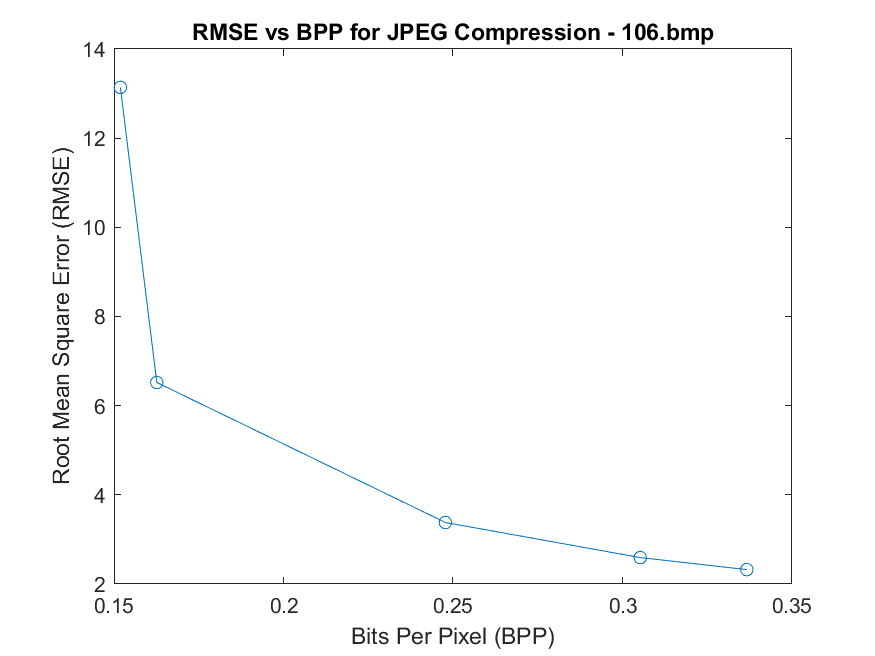
\includegraphics[width=0.7\textwidth]{images/106_rmse_vs_bpp.png}
    \caption{One instance of RMSE vs. Bits Per Pixel (BPP) for different quality factors.}
    \label{fig:rmse_bpp_plot}
\end{figure}

This document contains a reference to the images used in this analysis. You can access the photos at the following link:  
\href{https://drive.google.com/drive/folders/1rpRNlFg8iFSTTgFFgbw2oKc3_D-u5A7l?usp=drive_link}{\textbf{Photos on Google Drive}}.
\begin{table}
\centering
\caption{Comparison of Image Sizes}
\label{tab:image_sizes}
\begin{tabular}{llll}
\toprule
          Name & Original image size & Compressed size & Recovered size \\
\midrule
           106 &             14.4 MB &         1617 KB &        4802 KB \\
           108 &             14.4 MB &         1635 KB &        4802 KB \\
           109 &             14.4 MB &         1574 KB &        4802 KB \\
           111 &             14.4 MB &         1574 KB &        4802 KB \\
           112 &             14.4 MB &         1481 KB &        4802 KB \\
           114 &             14.4 MB &          1570KB &        4802 KB \\
          1697 &             9.18 MB &          984 KB &        3062 KB \\
          1698 &             9.18 MB &          793 KB &        3062 KB \\
          1714 &             9.18 MB &          977 KB &        3062 KB \\
  barbara\_grey &              258 KB &          299 KB &         258 KB \\
    camera man &              257 KB &          174 KB &         258 KB \\
         house &              513 KB &          186 KB &         514 KB \\
      jetplane &              513 KB &          247 KB &         514 KB \\
          lake &              513 KB &          308 KB &         514 KB \\
 lena\_grey\_512 &              258 KB &           63 KB &         258 KB \\
 lena\_gray\_256 &               65 KB &          190 KB &          66 KB \\
   living room &              257 KB &          245 KB &         258 KB \\
 mandrill\_gray &              257 KB &          327 KB &         258 KB \\
  peppers\_grey &              513 KB &          229 KB &         514 KB \\
        pirate &              257 KB &          242 KB &         258 KB \\
    walkbridge &              513 KB &          389 KB &         518 KB \\
  woman\_blonde &              257 KB &          211 KB &         258 KB \\
woman\_darkhair &              257 KB &          137 KB &         258 KB \\
\bottomrule
\end{tabular}
\end{table}

\subsection{Discussion}
The algorithm performs well in reducing file size while maintaining acceptable image quality. However:
\begin{itemize}
    \item \textbf{Strengths:} 
    \begin{itemize}
        \item Efficient use of frequency domain for compression.
        \item Effective reduction in redundancy using RLE and Huffman encoding.
        \item Customizable quality factor allows flexible trade-offs.
    \end{itemize}
    \item \textbf{Weaknesses:}
    \begin{itemize}
        \item High computational overhead due to block-wise DCT and Huffman encoding.
        \item Loss of detail in high-frequency regions at low quality factors.
        \item Limited optimization for real-time applications.
        \item Fixed quantization matrix limits adaptability.
    \end{itemize}
\end{itemize}

\section{Conclusion}
The implemented JPEG-like compression algorithm successfully demonstrates the principles of lossy image compression. The RMSE and BPP results confirm the effectiveness of the approach in achieving a balance between image quality and compression ratio. Future work could involve:
\begin{itemize}
    \item Extending the implementation to color images.
    \item Incorporating advanced entropy coding techniques like arithmetic coding.
    \item Optimizing the algorithm for real-time processing.
\end{itemize}

\end{document}